\begin{tikzpicture}[remember picture, scale=\modDGHyperScale]
% dummy
\coordinate[overlay] (\modIdPrefix v-coord-0-0) at (4.4297, 5.1408) {};
\coordinate[overlay] (\modIdPrefix v-coord-5-0) at (7.1853, 3.515) {};
\coordinate[overlay] (\modIdPrefix v-coord-8-0) at (3.6015, 2.4517) {};
\coordinate[overlay] (\modIdPrefix v-coord-15-0) at (1.4339, 8.1596) {};
\coordinate[overlay] (\modIdPrefix v-coord-24-0) at (10.469, 4.4999) {};
\coordinate[overlay] (\modIdPrefix v-coord-25-0) at (5.1712, 8.5591) {};
\coordinate[overlay] (\modIdPrefix v-coord-23-0) at (1.0729, 4.5781) {};
\coordinate[overlay] (\modIdPrefix v-coord-30-0) at (7.6017, 0.46108) {};
\coordinate[overlay] (\modIdPrefix v-coord-48-0) at (7.4075, 6.7159) {};
\coordinate[overlay] (\modIdPrefix v-coord-0-0-IOFlow) at (4.6919, 0.025) {};
\coordinate[overlay] (\modIdPrefix v-coord-5-0-IOFlow) at (10.561, 0.66333) {};
\coordinate[overlay] (\modIdPrefix v-coord-8-0-IOFlow) at (1.091, 0.52566) {};
\coordinate[overlay] (\modIdPrefix v-coord-24-0-IOFlow) at (10.15, 8.3305) {};

% id = 0, graphName = Ribulose-5-Phosphate
\node[modStyleDGHyperVertex, at=(v-coord-0-0)] (v-0-0) {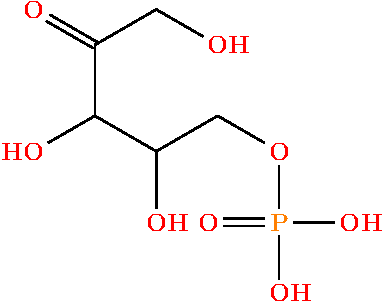
\includegraphics[scale=\modDGHyperImageScale] {\modInputPrefix/out/004_g_0_11311100.pdf}\\{$\mathrm{Ribulose-5-Phosphate}$}};
% id = 1, graphName = H2O
% id = 2, graphName = p_{25,0}
\node[modStyleDGHyperVertex, at=(v-coord-2-0)] (v-2-0) {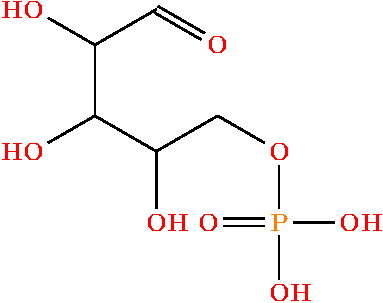
\includegraphics[scale=\modDGHyperImageScale] {\modInputPrefix/out/006_g_166_11311100.pdf}\\{$\mathrm{p_{25,0}}$}};
% id = 4, graphName = p_{25,1}
\node[modStyleDGHyperVertex, at=(v-coord-4-0)] (v-4-0) {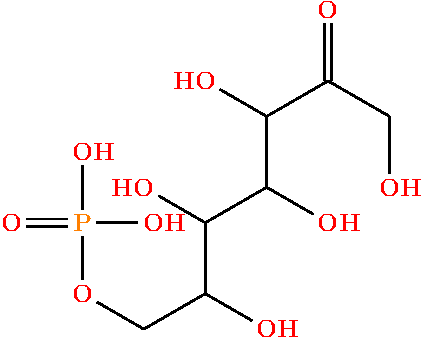
\includegraphics[scale=\modDGHyperImageScale] {\modInputPrefix/out/008_g_168_11311100.pdf}\\{$\mathrm{p_{25,1}}$}};
% id = 5, graphName = p_{25,2}
\node[modStyleDGHyperVertex, at=(v-coord-5-0)] (v-5-0) {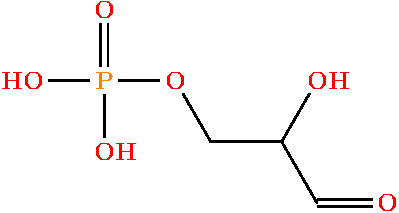
\includegraphics[scale=\modDGHyperImageScale] {\modInputPrefix/out/010_g_169_11311100.pdf}\\{$\mathrm{p_{25,2}}$}};
% id = 7, graphName = p_{25,3}
% id = 8, graphName = p_{25,4}
\node[modStyleDGHyperVertex, at=(v-coord-8-0)] (v-8-0) {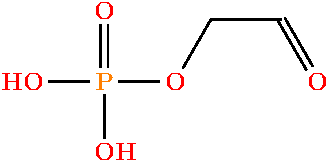
\includegraphics[scale=\modDGHyperImageScale] {\modInputPrefix/out/012_g_173_11311100.pdf}\\{$\mathrm{p_{25,4}}$}};
% id = 10, graphName = p_{25,5}
% id = 12, graphName = p_{25,6}
% id = 15, graphName = p_{25,7}
% id = 18, graphName = p_{25,8}
% id = 24, graphName = Fructose-6-Phosphate
\node[modStyleDGHyperVertex, at=(v-coord-24-0)] (v-24-0) {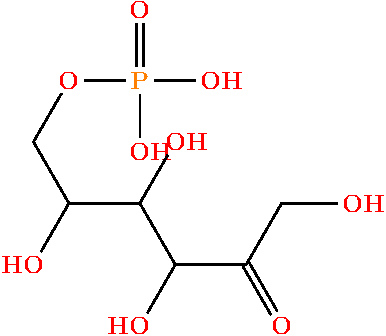
\includegraphics[scale=\modDGHyperImageScale] {\modInputPrefix/out/014_g_2_11311100.pdf}\\{$\mathrm{Fructose-6-Phosphate}$}};
% id = 25, graphName = p_{25,9}
\node[modStyleDGHyperVertex, at=(v-coord-25-0)] (v-25-0) {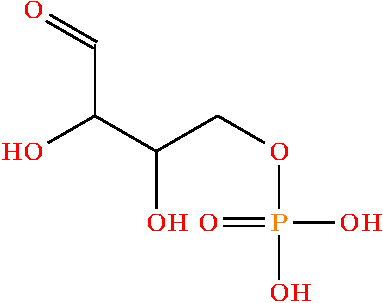
\includegraphics[scale=\modDGHyperImageScale] {\modInputPrefix/out/016_g_203_11311100.pdf}\\{$\mathrm{p_{25,9}}$}};
% id = 6{ 'Ribulose-5-Phosphate' 'p_{25,0}' }, 'Transketolase', { 'p_{25,1}' 'p_{25,2}' }
\node[modStyleDGHyperEdge, at=(v-coord-6-0)] (v-6-0) {$\mathrm{f\ 15,\ r_{2}}$};
% id = 27{ 'p_{25,1}' 'p_{25,4}' }, 'Transaldolase', { 'Ribulose-5-Phosphate' 'p_{25,9}' }
\node[modStyleDGHyperEdge, at=(v-coord-27-0)] (v-27-0) {$\mathrm{f\ 15,\ r_{3}}$};
% id = 30{ 'Ribulose-5-Phosphate' 'p_{25,2}' }, 'Transaldolase', { 'Fructose-6-Phosphate' 'p_{25,4}' }
\node[modStyleDGHyperEdge, at=(v-coord-30-0)] (v-30-0) {$\mathrm{f\ 30,\ r_{3}}$};
% id = 48{ 'Ribulose-5-Phosphate' 'p_{25,9}' }, 'Transketolase', { 'Fructose-6-Phosphate' 'p_{25,2}' }
\node[modStyleDGHyperEdge, at=(v-coord-48-0)] (v-48-0) {$\mathrm{f\ 15,\ r_{2}}$};
% id = 3{ 'Ribulose-5-Phosphate' }, 'Aldose-Ketose <-', { 'p_{25,0}' }
\path[modStyleDGHyperConnector] (v-0-0) to node[auto, swap] {$\mathrm{f\ 15,\ r_{0}}$} (v-2-0);
% id = 6{ 'Ribulose-5-Phosphate' 'p_{25,0}' }, 'Transketolase', { 'p_{25,1}' 'p_{25,2}' }
\path[modStyleDGHyperConnector] (v-0-0) to (v-6-0);
\path[modStyleDGHyperConnector] (v-2-0) to (v-6-0);
\path[modStyleDGHyperConnector] (v-6-0) to (v-4-0);
\path[modStyleDGHyperConnector] (v-6-0) to (v-5-0);
% id = 9{ 'Ribulose-5-Phosphate' 'p_{25,0}' }, 'Transaldolase', { 'p_{25,3}' 'p_{25,4}' }
% id = 11{ 'p_{25,1}' }, 'Aldose-Ketose <-', { 'p_{25,5}' }
% id = 13{ 'p_{25,3}' }, 'Aldose-Ketose <-', { 'p_{25,6}' }
% id = 14{ 'p_{25,1}' 'p_{25,2}' }, 'Transketolase', { 'Ribulose-5-Phosphate' 'p_{25,0}' }
% id = 16{ 'p_{25,1}' 'p_{25,4}' }, 'Transketolase', { 'p_{25,0}' 'p_{25,7}' }
% id = 17{ 'p_{25,0}' 'p_{25,1}' }, 'Transketolase', { 'p_{25,0}' 'p_{25,1}' }
% id = 19{ 'p_{25,2}' 'p_{25,3}' }, 'Transketolase', { 'Ribulose-5-Phosphate' 'p_{25,8}' }
% id = 20{ 'Ribulose-5-Phosphate' 'p_{25,2}' }, 'Transketolase', { 'Ribulose-5-Phosphate' 'p_{25,2}' }
% id = 21{ 'p_{25,3}' 'p_{25,4}' }, 'Transketolase', { 'p_{25,7}' 'p_{25,8}' }
% id = 22{ 'p_{25,0}' 'p_{25,3}' }, 'Transketolase', { 'p_{25,1}' 'p_{25,8}' }
% id = 23{ 'Ribulose-5-Phosphate' 'p_{25,4}' }, 'Transketolase', { 'p_{25,2}' 'p_{25,7}' }
% id = 26{ 'p_{25,1}' 'p_{25,2}' }, 'Transaldolase', { 'Fructose-6-Phosphate' 'p_{25,9}' }
% id = 27{ 'p_{25,1}' 'p_{25,4}' }, 'Transaldolase', { 'Ribulose-5-Phosphate' 'p_{25,9}' }
\path[modStyleDGHyperConnector] (v-4-0) to (v-27-0);
\path[modStyleDGHyperConnector] (v-8-0) to (v-27-0);
\path[modStyleDGHyperConnector] (v-27-0) to (v-0-0);
\path[modStyleDGHyperConnector] (v-27-0) to (v-25-0);
% id = 28{ 'p_{25,0}' 'p_{25,1}' }, 'Transaldolase', { 'p_{25,3}' 'p_{25,9}' }
% id = 29{ 'p_{25,2}' 'p_{25,3}' }, 'Transaldolase', { 'Fructose-6-Phosphate' 'p_{25,0}' }
% id = 30{ 'Ribulose-5-Phosphate' 'p_{25,2}' }, 'Transaldolase', { 'Fructose-6-Phosphate' 'p_{25,4}' }
\path[modStyleDGHyperConnector] (v-0-0) to (v-30-0);
\path[modStyleDGHyperConnector] (v-5-0) to (v-30-0);
\path[modStyleDGHyperConnector] (v-30-0) to (v-8-0);
\path[modStyleDGHyperConnector] (v-30-0) to (v-24-0);
% id = 31{ 'p_{25,3}' 'p_{25,4}' }, 'Transaldolase', { 'Ribulose-5-Phosphate' 'p_{25,0}' }
% id = 32{ 'p_{25,0}' 'p_{25,3}' }, 'Transaldolase', { 'p_{25,0}' 'p_{25,3}' }
% id = 33{ 'Ribulose-5-Phosphate' 'p_{25,4}' }, 'Transaldolase', { 'Ribulose-5-Phosphate' 'p_{25,4}' }
% id = 34{ 'p_{25,7}' }, 'Aldose-Ketose <-', { 'p_{25,9}' }
% id = 35{ 'Fructose-6-Phosphate' }, 'Aldose-Ketose <-', { 'p_{25,8}' }
% id = 36{ 'p_{25,7}' 'p_{25,8}' }, 'Transketolase', { 'p_{25,3}' 'p_{25,4}' }
% id = 37{ 'p_{25,7}' 'p_{25,9}' }, 'Transketolase', { 'Fructose-6-Phosphate' 'p_{25,4}' }
% id = 38{ 'p_{25,0}' 'p_{25,7}' }, 'Transketolase', { 'p_{25,1}' 'p_{25,4}' }
% id = 39{ 'p_{25,2}' 'p_{25,7}' }, 'Transketolase', { 'Ribulose-5-Phosphate' 'p_{25,4}' }
% id = 40{ 'p_{25,4}' 'p_{25,7}' }, 'Transketolase', { 'p_{25,4}' 'p_{25,7}' }
% id = 41{ 'Fructose-6-Phosphate' 'p_{25,8}' }, 'Transketolase', { 'p_{25,3}' 'p_{25,9}' }
% id = 42{ 'p_{25,1}' 'p_{25,8}' }, 'Transketolase', { 'p_{25,0}' 'p_{25,3}' }
% id = 43{ 'p_{25,3}' 'p_{25,8}' }, 'Transketolase', { 'p_{25,3}' 'p_{25,8}' }
% id = 44{ 'Ribulose-5-Phosphate' 'p_{25,8}' }, 'Transketolase', { 'p_{25,2}' 'p_{25,3}' }
% id = 45{ 'Fructose-6-Phosphate' 'p_{25,9}' }, 'Transketolase', { 'Fructose-6-Phosphate' 'p_{25,9}' }
% id = 46{ 'p_{25,1}' 'p_{25,9}' }, 'Transketolase', { 'Fructose-6-Phosphate' 'p_{25,0}' }
% id = 47{ 'p_{25,3}' 'p_{25,9}' }, 'Transketolase', { 'Fructose-6-Phosphate' 'p_{25,8}' }
% id = 48{ 'Ribulose-5-Phosphate' 'p_{25,9}' }, 'Transketolase', { 'Fructose-6-Phosphate' 'p_{25,2}' }
\path[modStyleDGHyperConnector] (v-0-0) to (v-48-0);
\path[modStyleDGHyperConnector] (v-25-0) to (v-48-0);
\path[modStyleDGHyperConnector] (v-48-0) to (v-5-0);
\path[modStyleDGHyperConnector] (v-48-0) to (v-24-0);
% id = 49{ 'Fructose-6-Phosphate' 'p_{25,0}' }, 'Transketolase', { 'p_{25,1}' 'p_{25,9}' }
% id = 50{ 'Fructose-6-Phosphate' 'p_{25,2}' }, 'Transketolase', { 'Ribulose-5-Phosphate' 'p_{25,9}' }
% id = 51{ 'Fructose-6-Phosphate' 'p_{25,4}' }, 'Transketolase', { 'p_{25,7}' 'p_{25,9}' }
% id = 52{ 'Fructose-6-Phosphate' 'p_{25,9}' }, 'Transaldolase', { 'p_{25,1}' 'p_{25,2}' }
% id = 53{ 'p_{25,1}' 'p_{25,9}' }, 'Transaldolase', { 'p_{25,1}' 'p_{25,9}' }
% id = 54{ 'p_{25,3}' 'p_{25,9}' }, 'Transaldolase', { 'p_{25,0}' 'p_{25,1}' }
% id = 55{ 'Ribulose-5-Phosphate' 'p_{25,9}' }, 'Transaldolase', { 'p_{25,1}' 'p_{25,4}' }
% id = 56{ 'Fructose-6-Phosphate' 'p_{25,0}' }, 'Transaldolase', { 'p_{25,2}' 'p_{25,3}' }
% id = 57{ 'Fructose-6-Phosphate' 'p_{25,2}' }, 'Transaldolase', { 'Fructose-6-Phosphate' 'p_{25,2}' }
% id = 58{ 'Fructose-6-Phosphate' 'p_{25,4}' }, 'Transaldolase', { 'Ribulose-5-Phosphate' 'p_{25,2}' }
% inFlow/outFlow, id = 0-0, graphName = Ribulose-5-Phosphate, inFlow = 60, outFlow = 0
\node[modStyleDGHyperVertexHiddenLarge, at=(v-coord-0-0-IOFlow)] (v-0-0-IOFlow) {};
\path[modStyleDGHyperConnector] (v-0-0-IOFlow) to node[auto, swap] {$\mathrm{f\ 60}$} (v-0-0);
% inFlow/outFlow, id = 8-0, graphName = p_{25,4}, inFlow = 0, outFlow = 15
\node[modStyleDGHyperVertexHiddenLarge, at=(v-coord-8-0-IOFlow)] (v-8-0-IOFlow) {};
\path[modStyleDGHyperConnector] (v-8-0) to node[auto, swap] {$\mathrm{f\ 15}$} (v-8-0-IOFlow);
% inFlow/outFlow, id = 24-0, graphName = Fructose-6-Phosphate, inFlow = 0, outFlow = 45
\node[modStyleDGHyperVertexHiddenLarge, at=(v-coord-24-0-IOFlow)] (v-24-0-IOFlow) {};
\path[modStyleDGHyperConnector] (v-24-0) to node[auto, swap] {$\mathrm{f\ 45}$} (v-24-0-IOFlow);
\end{tikzpicture}%
